\chapter{Einleitung}
\label{einleitung_cha}
\todo[inline]{Author hinzufügen}
\authorsection{Kinect-Gruppe}
Das aktuelle Interesse in der Forschung zur Robotik und insbesondere der Servicerobotik ist, Robotersysteme flexibler zu gestalten und für breitere Anwendungsgebiete, zum Beispiel statt eines reinen Staubsaugroboters einen Haushaltsroboter zu verwenden.
Im Fokus steht außerdem, wie auch in der Informationstechnologie, eine kostengünstige Verbesserung des Mensch-Maschine-Interface.
 \citep{IP08}

Die Forschungsfelder in Industrie- und Servicerobotik nähern sich dabei im Laufe der Jahre immer weiter an.
 So müssen Industrieroboter in Zusammenarbeit mit dem Menschen ihre Aufgaben verrichten und Serviceroboter
 in Zukunft auch komplexe Handhabungsaufgaben lösen. Die Entwicklung findet daher besonders im Bereich der
 Informationstechnologie und der Sensorik statt \citep{Michael2010}.
 
In den letzten Jahrzehnten hat sich die Bildverarbeitung rasant weiterentwickelt.
 Zur meist funktionsrelevanten Interaktion eines Serviceroboters mit der Umwelt muss
 ein Roboter aufgrund der Vielfalt möglicher Umgebungen adaptiv in der Lage sein, reichhaltige
 Informationen darüber zu gewinnen. Unstrukturierte Umgebungen lassen sich nicht vollständig modellieren.
 Roboter müssen somit durch Interaktion mit ihrer Umwelt lernen, sich orientieren und auf Menschen bzw. Informationen reagieren.
 Besonders anspruchsvoll sind dabei Perzeption und Verarbeitung von Signalen.

\section{Motivation und Problemstellung}
\label{motivation_sec}
\todo[inline]{Author hinzufügen}
\authorsection{Kinect-Gruppe}

In vielen Fällen müssen sich Serviceroboter in unstrukturierten Umgebungen zurechtfinden, in denen es nicht möglich ist, diese durch
 (zum Beispiel markerbasierte) spezielle Kennzeichnung der Objekte mit Informationen anzureichern \citep{sturm10rss-workshop}.
 Auch Industrieroboter sollen in Zukunft enger mit (unberechenbaren) menschlichen Kooperationspartnern zusammenarbeiten.
 Kamerabilder stellen in diesem Kontext eine reichhaltige und kostengünstige Informationsquelle dar und können über Sensorfusion bzw. Musterprojektion zusätzlich
 zu 3D-Tiefenbildern erweitert werden. 

Das Identifizieren und Verfolgen geometrischer Objekte in (Tiefen-) Bildern ist ein weit entwickeltes Feld mit hoher Reife und etablierten Methoden.
 Die große Herausforderung ist die semantische Interpretation dieser Daten. Besonders das zuverlässige Gewinnen funktionsrelevanter Informationen,
 wie zum Beispiel interaktiver Charakteristika, kinematischer, werkstofftechnischer und  Oberflächen-Beschaffenheit aus (Tiefen-) Bildern stellt sich
 als problematisch dar. In unstrukturierten Umgebungen jedoch versagen andere Sensorentypen oder deren Anwendung ist bisher aufgrund des Preises sinnlos.
 
Aktuell werden verschiedene Ansätze verfolgt: Zum einen generiert und erfasst man weitere Sensorinformationen durch Interaktion eines Roboters mit der Umgebung,
 zum anderen werden dem Roboter weitreichende erwartete Zusammenhänge von Informationen bereitgestellt. Entwickler können bei diesen Aufgaben auf weit entwickelte Roboterplattformen
 zurückgreifen, wie den PR2 der Firma willow garage und wie in diesem Praktikum
 \gls{hollie} des \gls{fzi} Karlsruhe. Willow garage stellt auch umfangreiche
 Software zur (Tiefen-) Bildverarbeitung und Robotersteuerung zur Verfügung,
 wie \gls{opencv}, \gls{pcl} und \gls{ros}.

\section{Stand der Technik}
\label{stand_der_technik_sec}
\todo[inline]{Author hinzufügen}
\authorsection{Kinect-Gruppe}

\subsection{Hardware}
\subsubsection{3D Kameras (am Beispiel Microsoft Kinect)}
Die Abbildung \ref{fig:Kinect} zeigt ein Bild der Kinect. Sie ist mit
 laser-basiertem \gls{ir} Projektor und einem monochromen \gls{cmos} Sensor ausgestattet.
 Der \gls{ir}-Projektor projiziert ein Muster auf die beobachtete Szenerie,
 während der \gls{cmos} Sensor die Verformungen des Musters detektiert und gegen
 ein Vorgabemuster mittels Epipolargeometrie ein Tiefenbild errechnet.
 Die Kinect ist darüber hinaus mit einem Neigemotor, einer Reihe von Mikrofonen
 und einer \gls{rgb}-Kamera ausgestattet. Horizontal hat die Kamera einen Öffnungswinkel
 von $57^\circ$ und vertikal $43^\circ$. Die Arbeitsentfernung der Kinect liegt
 zwischen $0,8$ und $3,5m$. Die Auflösung der Tiefenkamera beträgt $3mm$ in
 der X/Y Ebene und $10mm$ in Z-Richtung bei einem Abstand von $2$ Metern. Die
 Auflösung ist $640$ x $480$ Bildpunkte bei einer Bildfrequenz von $30Hz$. Das
 Tiefenbild hat eine $11bit$ Auflösung mit Werten zwischen $0$ und $2047$.

\begin{figure}[h]
\center
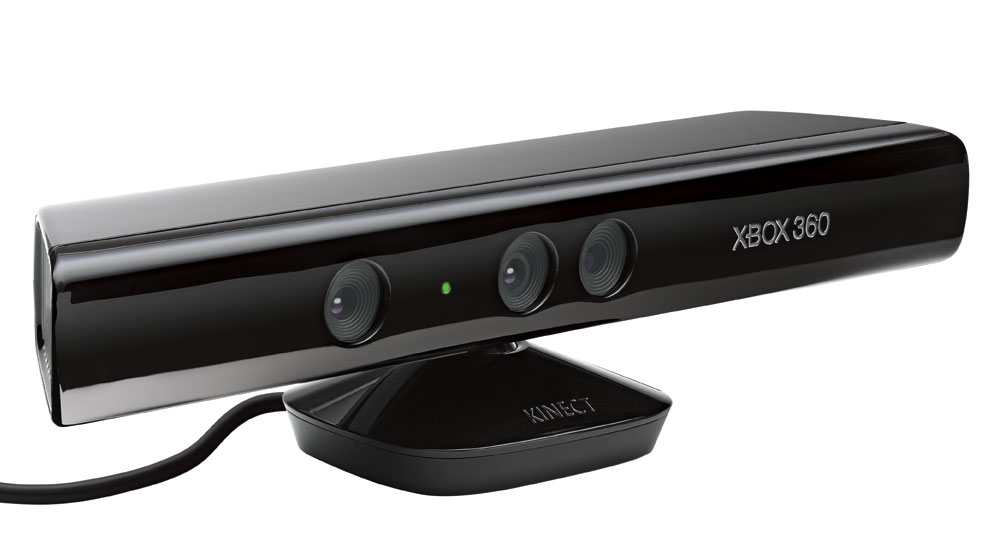
\includegraphics[scale=0.3]{graphics/Kinect.jpg}
\caption{\label{fig:Kinect} Kinect}
\end{figure}
\todo{Quelle des Kinect-Bilds??}

Für die Kinect wurden in den letzten Jahren mehrere Entwicklerbibliotheken erstellt,
 die sich wachsender Beliebtheit erfreuen. Es ist eine rasant wachsende Anzahl von Applikationen vorhanden,
 die 3D Kameras unterstützen. Ursprünglich als Entertainmenthardware entwickelt,
 findet die Kinect vermehrt auch in der Forschung massiv Anwendung.
 Ähnliche Spezifikationen haben auch die Wavi Xtion Kamras der Firma ASUS.

\subsubsection{Mobile Roboterplattformen}

Mobile Roboterplattformen werden in den meisten Fällen zu Forschungszwecken verwendet.
 Wissenschaftler verschiedener Disziplinen wirken an Design und Programmierung mit.
 Sie weisen teils stark unterschiedliche Konfigurationen auf.
 Seit vielen Jahren wird jedoch intensiv an menschenähnliche Prototypen gearbeitet.
 Nach der Konstruktion dienen solche Plattformen häufig dazu, durch verschiedenste Programmierungen
 vorgegebene Aufgaben zu erfüllen. Im Rahmen des Mobile Roboterpraktikums haben
 wir an der Plattform \gls{hollie} des \gls{fzi} Karlsruhe gearbeitet. Auch die
 Roboterplattform ARMAR wurde in Karlsruhe am \gls{kit} entwickelt.
 Aufgrund der großen Popularität, technischen Ausgereiftheit und guten
 Dokumentation soll jedoch exemplarisch an dieser Stelle die Roboterplattform
 PR2 der Firma willow garage dargestellt werden, siehe Abbildung
 \ref{fig:PR2Struktur}.

\begin{figure}[h]
\center
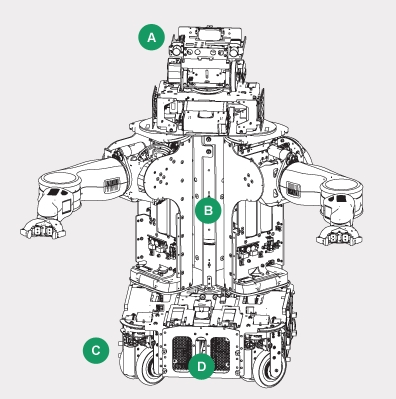
\includegraphics[scale=0.5]{graphics/PR2Struktur.jpg}
\caption{\label{fig:PR2Struktur} Struktur des PR2 \citep{hspecsWG2012}}
\end{figure}

Der PR2 ist ein kommerziell erhältlicher, weit entwickelter humanoider Roboter, der den typische Aufbau humanoider Roboterplattformen aufweist.
 Er hat folgende, \gls{hollie} ähnlicher, technische Eigenschaften \citep{hspecsWG2012}:

\begin{itemize}
  \item 2 Arme mit Greifern (Arm 4 \gls{dof}, Handgelenk 3 \gls{dof}, Greifer 1 \gls{dof})
  \item Kopf mir 2 \gls{dof}
  \item Omnidirektionale Basis (3 \gls{dof})
\end{itemize}

Außerdem ist der PR2 mit einer großen Anzahl an Sensoren ausgestattet
 ist und innerhalb gewisser Parameter modular konfiguriebar.
 Der PR2 ist mit folgenden Sensoren ausgestattet bzw. ausstattbar:

\begin{itemize}
  \item Microsoft Kinect
  \item 5 MP Kamera
  \item Stereokamerasystem
  \item Kleinwinkelkamera
  \item \gls{led} Musterrojektor
  \item Laserscanner
  \item Mikrofonarray
  \item Beschleunigungssensorik in den Armen
  \item Kraftsensorik in den Greifern
  \item Kalibrierungs-\glspl{led}
\end{itemize}

Der PR2 wird mittlerweile an einigen namhaften Universitäten und Forschungsstätten eingesetzt
 (u.a. \gls{tu} München, Stanford University und \gls{mit}) und es existieren Arbeiten in verschiedensten Bereichen,
 wie zur Betreuung älterer und eingeschränkter Menschen, zum Verrichten von Hausarbeiten  und dem Einsatz
 in Dienstleistungsbetrieben.

Besonders an dem Roboter ist die gemeinsame mechatronische, aber besonders informationstechnische Plattform,
 die auf dem Betriebssystem \gls{ros} aufbaut und es Wissenschaftlern
 ermöglicht in einer gemeinsamen Umgebung zu arbeiten, Ergebnisse auszutauschen und auf neue Generationen zu übertragben.

\subsection{Software}

\subsubsection{OpenNI}

\gls{openni} ist ein plattformübergreifendes Framework zur Entwicklung von
Applikationen, die auf natürlicher Mensch-Maschine-Interaktion aufbauen.
 Die \gls{openni}-\gls{api} stellt eine Vielzahl an Schnittstellen bereit, um
 entsprechende Applikationen zu programmieren. Der Hauptzweck von \gls{openni}
  ist eine Standard-\gls{api} bereitzustellen, die folgende Eigenschaften vereint \citep{openNI2012}:

\begin{itemize}
  \item Kommunikation mit Video und Audiosensoren
  \item Bereitstellung von Middleware zur Video- und Audiodatenverarbeitung,\\
  wie die Unterstützung bei der Objektdetektion in Bildern
\end{itemize}

Dabei stellt \gls{openni} eine Reihe von \glspl{api} bereit, die sowohl von  (3D-Kamera-)
 Sensoren als auch Middleware Komponenten implementiert werden können.
 Durch das Entkoppeln von Sensor und Middleware können mit \gls{openni} angefertigte Softwareprodukte
 ohne zusätzliche Arbeit auf verschiedener Middleware aufbauen (\glqq write once, deploy everywhere\grqq).
 Middleware Entwickler können somit Algorithmen, die auf standardisierten (Bild-) Formaten aufbauen,
 unabhängig von der Sensorik-Hardware entwickeln. Hardware Hersteller müssen auf der anderen Seite
 Sensoren zur Verfügung stellen, die diese Bildformate generieren können. \gls{openni} steht kostenlos
 als open source Quelle zur Verfügung. In Abbildung \ref{fig:openNI} ist das
 Konzept von \gls{openni} in 3 Schichten dargestellt:

\begin{description}
  \item[Oben:] Software, die Natürliche Interaktion auf \gls{openni} aufbauend
  verwendet
  \item[Mitte:] \gls{openni}, das Kommunikationsschnittstellen sowohl zu
  Hardware- als auch zu\\ Softwarekomponenten zur Verfügung stellt
  \item[Unten:] Hardwarekomponenten, die Video- und Audiosignale aufnehmen
\end{description}

\begin{figure}[h]
\center
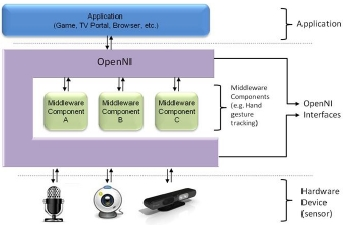
\includegraphics[scale=0.8]{graphics/openNI.jpg}
\caption{\label{fig:openNI} \gls{openni} Architektur \citep{openNI2012}}
\end{figure}

OpenNI basiert auf einigen Grundkonzepten:

\begin{itemize}
  \item Modularität
  \item Produktionsknoten
  \item Produktionsketten
\end{itemize}

\newpage
\todo[inline]{Ein wenig gepfuscht hier \ldots falls wer Lust hat kann er das
ja ändern}
\begin{description}
\item[Modularität]
\end{description}

Unter Modularität ist in diesem Zusammenhang vor allem die Austauschbarkeit von Komponenten
 und die Architektur des Systems zu verstehen.
 Es werden folgende Module unterstützt:


\begin{itemize}
\item \textbf{Sensoren:}
\begin{itemize}
  \item 3D Sensoren
  \item \gls{rgb} Kameras
  \item Infrarot Kameras
  \item Mikrofone / Mikrofonarrays
\end{itemize}
\item \textbf{Middleware Komponenten:}
\begin{description}
  \item[Ganzkörperanalyse Middleware:] Softwarekomponente, die Sensordaten
  verarbeitet und daraus relevante Informationen wie Gelenkposen ableitet
  \item[Handanalyse Middleware:] Software, die hilft Sensordaten zu verarbeiten,
  um die Positionen von Händen zu ermitteln
  \item[Gestendetektion:] Softwarekomponente, die Gesten erkennt und diese
  Information an die Anwendungen weitergibt
  \item[Szenenanalyse:] Software, die verschiedene Szenenrelevanten
  Informationen ableitet, wie Hintergrundseparation, Erkennen der Bodenebene und Identifikation und Detektion von verschiedenen Personen
\end{description}
\end{itemize}


\begin{description}
\item[Produktionsknoten]
\end{description}


In \gls{openni} werden sogenannte Produktionsknoten definiert die die Aufgabe haben,
 für verschiedene Anwendungen die Daten zur Verfügung zu stellen.
 Produktionsknoten stehen dabei in einer Hierarchie zueinander.
 Sie können sowohl Produktionsknoten eines niedrigeren Levels verwenden als auch von Knoten höheren
 Levels verwendet werden. Konkret bietet \gls{openni} einen User Generator, der alle Daten einer getrackten Person
 liefern kann. Hierfür verwendet der User Generator einen Tiefenbildgenerator, aus dem er seine Informationen ableitet.

\begin{description}
\item[Produktionsketten]
\end{description}

Wie bereits dargestellt können mehrere Module gleichzeitig an der selben \gls{openni} Distribution angemeldet sein.
 Diese Topologie erlaubt Anwendungen flexibel auf Aufnahme- und Verarbeitungsmodule zuzugreifen.
 Als Produktionsketten werden die bereits angesprochenen hierarchischen Verarbeitungsketten der Produktionsknoten verstanden.
 Der erwähnte User Generator verwendet einen Tiefengenerator, der wiederum seine Daten von einem Tiefensensor bezieht.
 Diese Abhängigkeit bzw. sequenzielle Herunterbrechen der Aufgabe der Produktionsknoten wird als Produktionskette verstanden.
 Vorteilhaft ist an dieser Struktur, dass Anwendungen nur die oberste Schicht mit ihren Fähigkeiten nutzt.
 Die Konfiguration der darunter liegenden Schichten bleibt dabei verborgen und erlaubt Herstellern größere Freiheit
 in der Gestaltung der niedrigeren Hierarchieebenen \citep{openNI2012}.

\subsubsection{Microsoft \glsentrytext{sdk}}

Auch der Hersteller der Kinect, Microsoft, bietet nun ein offizielles \gls{sdk},
 das sich leicht in Visual Studio und Dot Net integrieren lässt. Mit dem Kinect Sensor und Microsoft \gls{sdk}
 hat man Zugang zu Werkzeugen, mit denen Menschen und Sprache erkannt werden.
 Darüber hinaus existiert ein Entwicklerportal mit kostenlosen Tutorials und Beispielen.
 Dort kann Microsoft \gls{sdk} auch kostenlos heruntergeladen werden \citep{kinectDevKfW2012}.

Die Sprach- und Gestenerkennung findet nicht nur in Spielen sondern auch in der Bedienung des Computers Anwendung,
 wie zum Beispiel bei Microsofts Internetsuchmaschine bing\footnote{\url{www.bing.com/}}. Eine neu entwickelte Körperscan Software erlaubt es,
 Bilder aufzunehmen und diese als Animationen oder als Avatar in Spielen zu
 verwenden, siehe Abbildung \ref{fig:skelettracking} \citep{noGameKinect2012}.

\begin{figure}[h]
\center
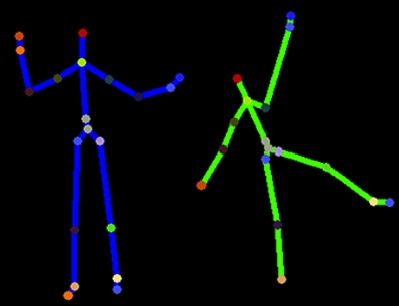
\includegraphics[scale=0.8]{graphics/skelettracking.jpg}
\caption{\label{fig:skelettracking} Beispielhafte Anwendung von Skelettracking
\citep{noGameKinect2012}}
\end{figure}
